\section{Evaluation Methodology}
\label{sec:evaluation}

The evaluation follows the security argument from implementation semantics to
commit-time consumption. We first characterize effect distinctions, then use
source-executed policy-separating pairs to falsify coarse interfaces and test
frozen candidates. Holding calls, state, authority, and decision logic fixed
isolates the authorization consequences of representation choice. Finally, an
AgentDojo study exercises a registered interface at an audited pre-commit
boundary.

\begin{table*}[t]
\centering
\scriptsize
\setlength{\tabcolsep}{3.5pt}
\caption{Evaluation evidence map. Each protocol supports one step of the
security argument; evidence from a later stage does not retroactively certify
an earlier one.}
\label{tab:evaluation-evidence-map}
\begin{tabular}{@{}p{0.13\textwidth}p{0.17\textwidth}p{0.21\textwidth}p{0.23\textwidth}p{0.20\textwidth}@{}}
\toprule
Stage & Domain & Purpose & Evidence / decision source & Supported claim \\
\midrule
Source characterization & AgentDojo benign trajectories & Establish compound and state-dependent implementation behavior & Copied-sandbox before/after execution & Tool identity and call text may omit committed distinctions \\
Interface falsification & 56-call source relation & Construct separating counterexamples & Source execution plus finite diagnostic policy relation & Coarse views are insufficient on witnessed pairs \\
Post-freeze check & 11 tools, three public MCP implementations & Test a frozen candidate on descriptor-blind contexts & Independent source execution plus native-delta policy & Candidate preserves the exercised distinctions \\
Explicit authority & Four domains, 1,024 contexts & Measure downstream authorization consequences and a strong state-aware alternative & ACL, capability, and delegation engine & Sufficiency depends on preserved distinctions, not a privileged syntax \\
Integration & 30 copied-sandbox trajectories; AgentDojo audit & Exercise pre-commit consumption and reconciliation & Explicit authority and native validators & A registered interface can be consumed at a check--use boundary \\
\bottomrule
\end{tabular}
\end{table*}

Table~\ref{tab:evaluation-evidence-map} maps each evidence source to the claim
it tests and the oracle that supplies its reference decision.
Figure~\ref{fig:evaluation-evidence-chain} visualizes the same chain.

\begin{figure*}[t]
\centering
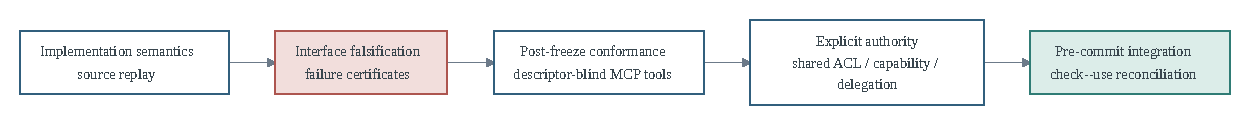
\includegraphics[width=\textwidth]{figures/mermaid_clean/pdf/fig_evaluation_evidence_chain.pdf}
\caption{Evaluation evidence chain. Each stage supplies one step of the
security argument; Table~\ref{tab:evaluation-evidence-map} gives the
corresponding domains, oracles, and claims.}
\label{fig:evaluation-evidence-chain}
\end{figure*}


\paragraph{Interpretation of evidence.}
The two result directions are asymmetric. One source-executed pair with
different ideal decisions and the same representation conclusively falsifies
that interface on any domain containing the pair. The absence of such a pair
creates a conformance record for the implementation, interventions, and policy
family used by the test. The artifact binds these elements and all
unresolved tests to each accepted descriptor.

Three evidence sources have distinct roles. The \emph{source execution oracle}
answers what the implementation committed in a copied pre-state. The
\emph{policy-separation oracle} determines whether two observed semantic views
require different decisions under the diagnostic policy family. The later
\emph{explicit-authority engine} is a concrete downstream consumer over ACLs,
capabilities, and delegations. These components establish implementation
behavior, policy relevance, and downstream consumption, respectively.

\paragraph{Implementation semantics.}
We replay all 339 calls in AgentDojo v1.1.2's 97 official benign trajectories
from fresh prescribed states. Before/after differences are normalized into
resource, target, visibility, message, membership, and external-interaction
effects. We count effect occurrences and cross-type or cross-subsystem calls. A
56-call source domain adds payload, temporal, recurrence, repeated-effect, and
state-dependent distinctions.

\paragraph{Interface falsification and post-freeze checking.}
The registration harness varies values, types, boundaries, list cardinality,
omitted defaults, and pre-state under a fixed implementation; surface changes
serve as invariance placebos. It classifies every attempt as a committed-effect
change, output-only change, invariant, invalid, or unresolved. A failure
certificate requires changed source behavior, a different policy decision, and
an unchanged candidate representation.

The 56-call analysis uses a finite source-effect/submultiset relation for
interface-discrimination stress, and a frozen initial set of 80 intervention
executions drives refinement. The later authority protocol supplies deployment-style policies.
For evidence from independently implemented tools, we pin a public filesystem
server, SQLite server, and graph-memory server at specific commits; these tools
belong to a public tool ecosystem whose security has been surveyed and
audited~\cite{hou2025mcplandscape,radosevich2025mcpaudit,gaire2025sokmcp}, and
whose manuals and schemas can be poisoned~\cite{liu2026manualiles}.
Their 11 stateful tools are selected outside our benchmark. Registration uses
12 counterfactual pairs per tool (24 registration contexts per tool, 264 in
total). We then freeze the descriptors and execute
24 descriptor-blind contexts per tool with disjoint values, states, and list
cardinalities. Each invocation runs the original MCP implementation in a fresh
disposable fixture. To isolate construction from evaluation, descriptors are
frozen before context generation, and the generator, source oracle, descriptor
compiler, and native-policy path are implemented as separate modules. The
native path derives decisions directly from raw filesystem, row, and graph
deltas; the typed path compiles the pre-commit request for the authority engine.
We compare tool name, raw call, state-aware request, common fields, typed
effects, and a diagnostic source-effect oracle. Each validation record includes
the implementation provenance.

Before evaluation outcomes are read, a mutation manifest deletes templates or
pre-state dependencies, disables list expansion, removes qualifier bindings,
swaps resource and target, collapses operations, or ignores no-op/default
behavior when applicable. Every mutant is tested during registration and on
the frozen descriptor-blind contexts. Mutants that change no decision in either
frozen domain are recorded as decision-equivalent there.

\paragraph{Authorization under explicit authority.}
The downstream experiment uses four copied-sandbox domains: calendar,
workspace sharing, messaging, and banking. Their authority state is expressed
as resource ACLs, channel capabilities, and attenuated transfer delegations.
The same tri-state engine consumes every representation. Calls, pre-states,
authenticated subjects, authority state, and decision logic remain fixed; only
the observation interface changes.

Registration executes 192 counterfactual pairs spanning resource, target,
operation mode, qualifier, default, pre-state, and surface-invariant changes.
The resulting typed-effect descriptors are hash-frozen and loaded as
executable JSON. Evaluation uses 1,024 contexts materialized after freeze from
a precommitted generator and authority configuration. The source transition
oracle and descriptor compiler are separate implementations. The explicit-authority engine evaluates the source-observed transition to
obtain the ideal decision. Each candidate representation is then compared
against that decision to identify mixed representation cells.

We compare the tool-name view, canonical raw-call view, common-field view, and
typed-effect interface. We additionally evaluate a state-aware request view
containing totalized arguments and ACL-relevant attributes of directly
referenced resources. Its collision track consists of this request view; a
hash-frozen adapter supplies the disclosed tool-specific operation knowledge required by
the shared authority engine. The raw-call view contains totalized call text,
whereas the state-aware view also exposes trusted pre-state attributes. Both are
evaluated under Definition~\ref{def:authorization-equivalence}.

We audit both consumption paths on the 1,024- and 264-context domains, recording
representation cells, source-equivalent overpartition, serialized size,
policy-facing trusted state, code structure, descriptor size, and staged
latency. Timing uses three warm-up and 30 complete measured batches.

\paragraph{Pre-commit integration.}
We first run 30 short trajectories over \texttt{schedule\_meeting},
\texttt{share\_document}, and \texttt{transfer\_funds}. The local Qwen3-32B
checkpoint proposes a structured call. The frozen descriptor instantiates effects, the
explicit-authority engine decides, and an allowed checked call executes in the copied
sandbox. Each commit is reconciled against both the checked call and observed
post-state transition.

AgentDojo supplies 97 benign tasks and 629 official indirect-injection pairs.
Under a fixed DeepSeek model (\texttt{deepseek-v4-flash}) and native
validators, repeated runs compare no guard,
Spotlighting~\cite{spotlighting2024}, and the provenance-origin consumer from
Section~\ref{sec:security-analysis}. A second common protocol runs no guard,
Spotlighting~\cite{spotlighting2024}, Prompt Sandwiching\footnote{We implement the sandwich-defense recipe documented at \url{https://learnprompting.org/docs/prompt_hacking/defensive_measures/sandwich_defense}; it is a prompting technique rather than a single citable paper.}, a PromptArmor-style
local adapter~\cite{promptarmor2025}, and the
consumer on the same Qwen3-32B checkpoint and exact 726 benchmark keys. Every
decision is reconciled with the executed call. Public-family and AgentLAB
saved-replay protocols test transfer, while a raw-field control measures
whether typed semantic roles alter runtime decisions.

\paragraph{Metrics and integrity.}
Interface tests report mixed cells and policy-separating pairs. The authority
experiment reports unsafe allow among ideal denials, authorized work withheld
among ideal allows, coverage, abstention, exact-decision rate, and the
unavoidable-error lower bound induced by mixed cells. A denial and an
abstention are distinct monitor outcomes, but either withholds an authorized
operation; coverage records how often the monitor commits to
\Allow{} or \Deny{}. Native benchmark validators compute runtime outcomes.
All protocols retain invalid and failed rows, run in copied or replayed
environments, and produce no external side effects.
Appendix~\ref{app:open-science} describes the fail-fast
reproduction checks.
